\appendix{Gen3 Software}
%\subappendix{Clinical Software}
\begin{figure}[h]
\centering
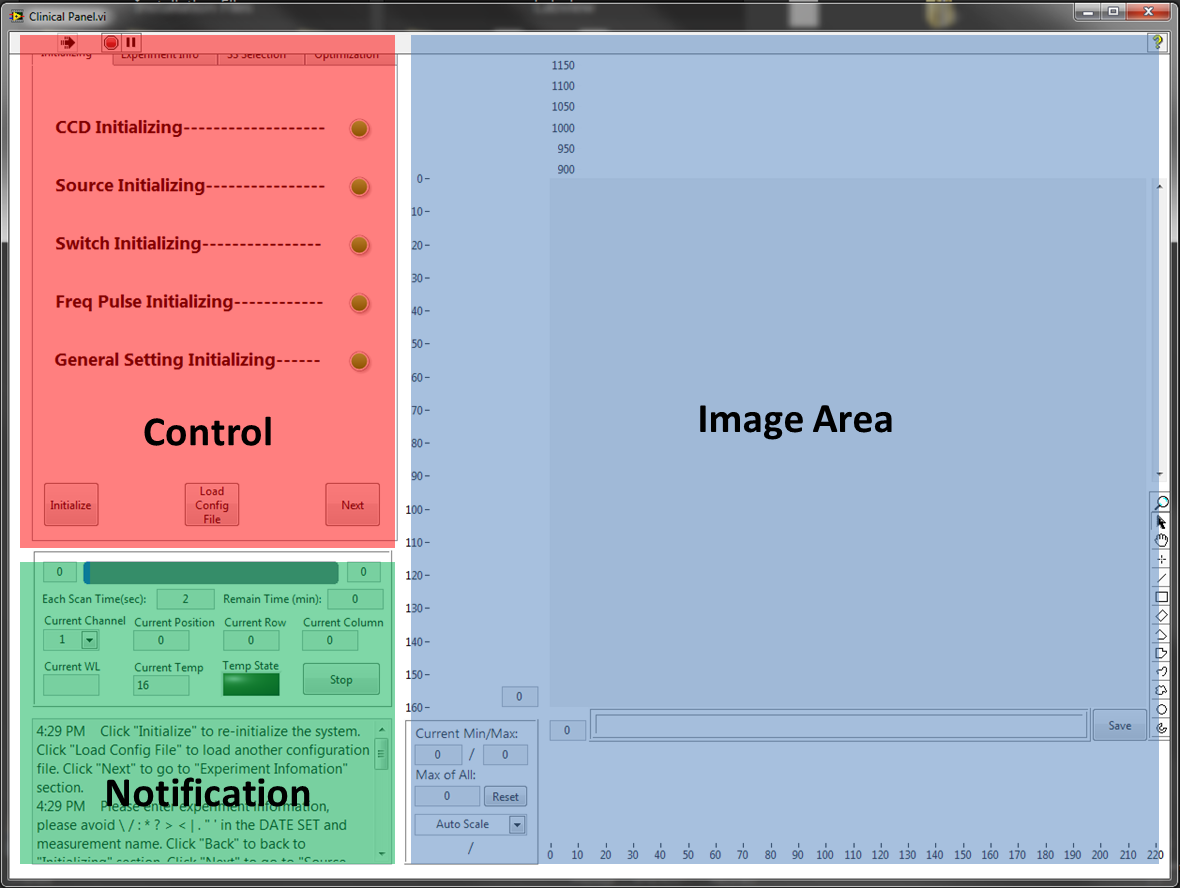
\includegraphics[width=13.5cm]{./figures/A_Gen3Software/Clinical1.png}
\caption[The Gen3 Clinical software written in Labview]{The Gen3 Clinical software written in Labview. The software consist of a control area (red) where the user interacts with the software, the notification area (area) where the instrument status and notifications are displayed, and the imaging area (blue) where the image from the Gen3 CCD is displayed.}
\label{fig:Clinical1}
\end{figure}
The Gen3 Clinical software was written with our clinical collaborators in mind. It minimizes access to the hardware and simplifies the measurement process to reduce user error. Figure~\ref{fig:Clinical1} shows the general layout of the software. The upper left area has the polymorphic interface controls (indicated in red) where the user mainly interacts with the software. Right below is the notification area (indicated in green) which displays the status of the instrument and various errors and notifications. Finally on the right is the image display (indicated in blue) where images from the Gen3 CCD is displayed.

The first panel that displays (Figure~\ref{fig:Clinical2}) is the initialization screen. Pressing the initialization button will do a system check of the CCD and the DAQ module.
\vspace{2mm}
\begin{figure}[bh]
\centering
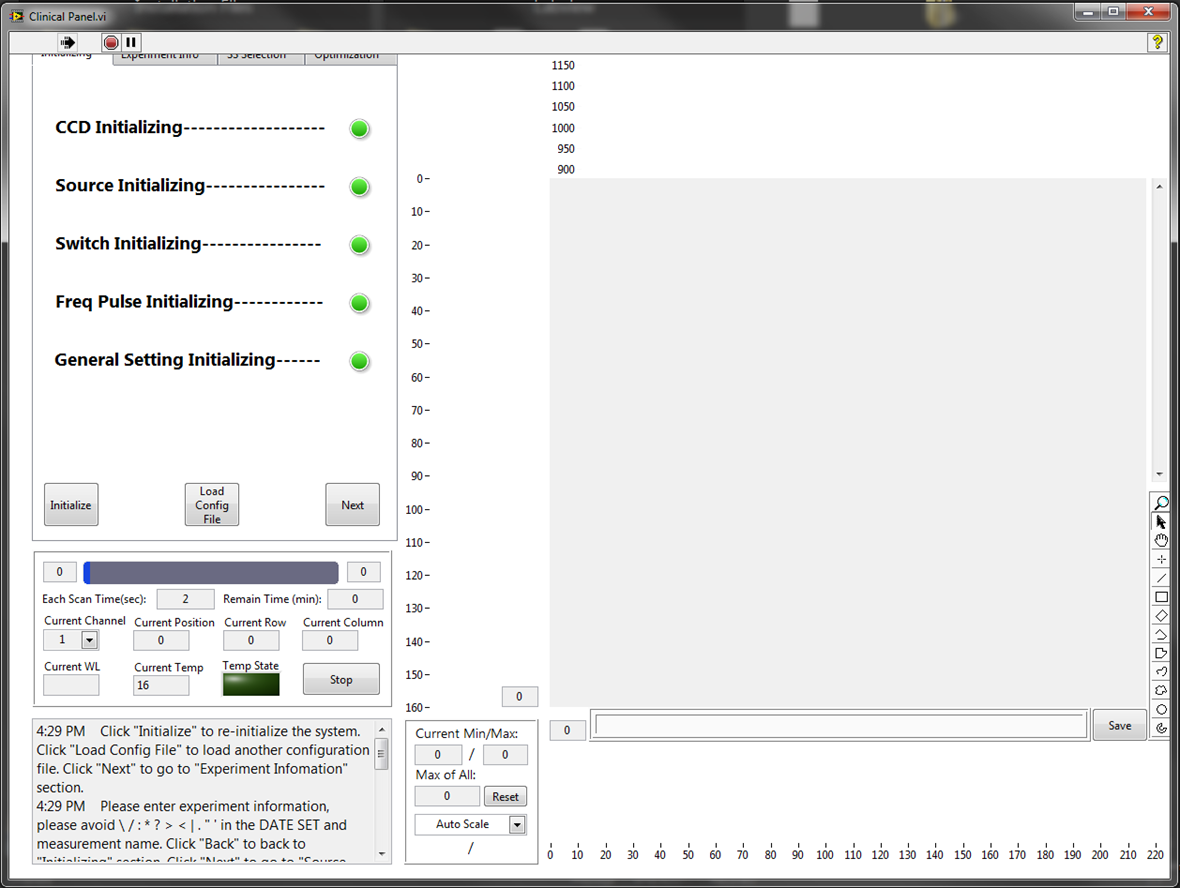
\includegraphics[width=13.5cm]{./figures/A_Gen3Software/Clinical2.png}
\caption[Initialization panel in the clinical software]{The first screen in the software is the initialization configuration screen. At this step, the hardware connection and statuses are checked before allowing the user to proceed. After the hardware status is checked, the user can load a preconfigured config file or proceed without one. The user can then continue onto the next step.}
\label{fig:Clinical2}
\end{figure}
If there are any errors or if these parts are disconnected, it will be indicated in the notification area. If all checks are successful and all green indicators are lit, the user can then load a configuration file (that has already been created in the Gen3 Experimental Software). Once a configuration file is loaded successfully, the user may proceed by clicking ``next". 

The proceeding screen is the Data input screen where the measurement details are recorded. The current date is automatically loaded and the control panel asks the user for the experiment number and the number of measurements. The minimum number of measurements is two: 1) one for the reference, and 2) one for a single breast measurement. The user can set up to 12 independent measurements before clicking ``next".
\begin{figure}[h]
\centering
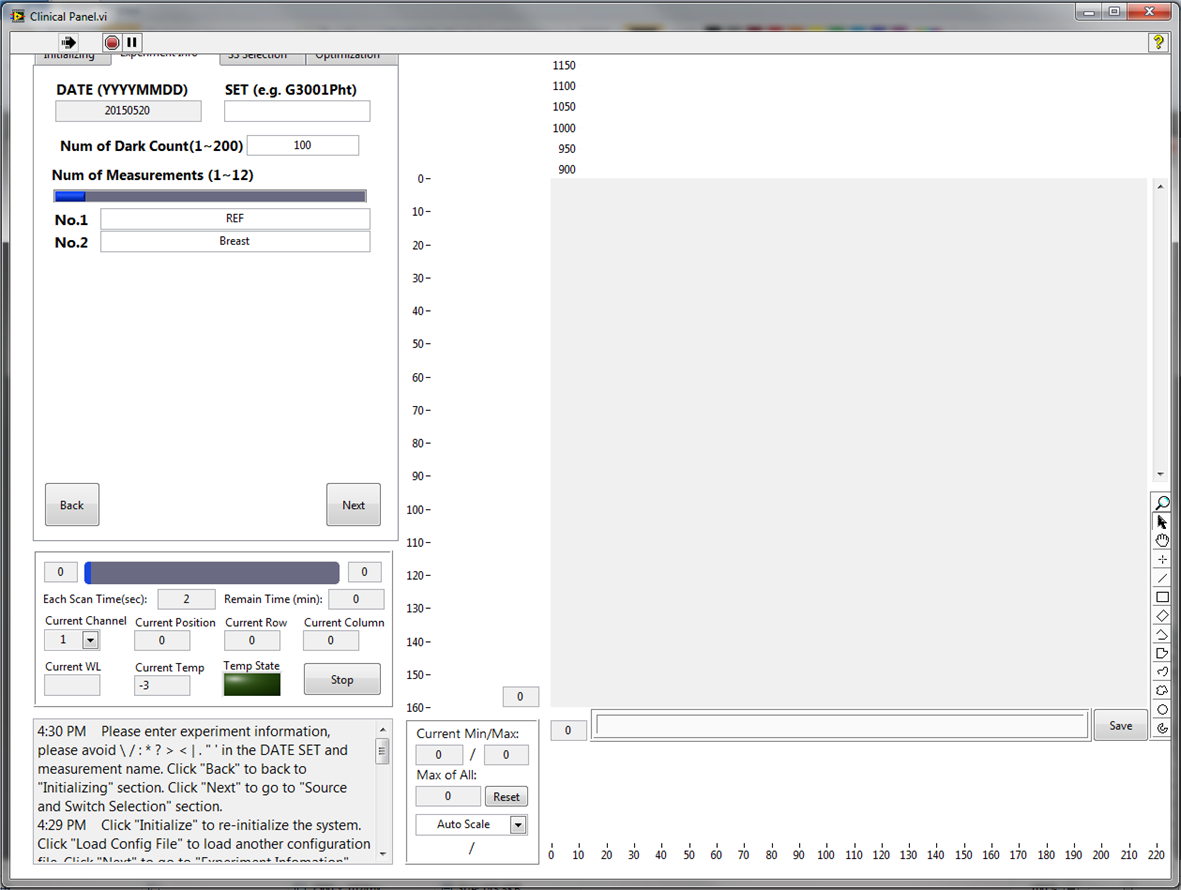
\includegraphics[width=13.5cm]{./figures/A_Gen3Software/Clinical3.png}
\caption[Measurement record panel in the clinical software]{The second panel is the Data input screen where the details of the measurement is entered. The patient number and the number of measurements can be indicated. The minimum number of measurements is two (typically for reference and a single breast measurement) but can be increased to 12.}
\label{fig:Clinical3}
\end{figure}

The third panel (Figure~\ref{fig:Clinical4}) in the clinical software is the source configuration screen. Here the user can choose the sources and wavelengths that will be used for the measurement. The first $11\times19$ indicators are for the source position. The second $11\times19$ grid is the calibration source grid. The user can indicate after which source the calibration measurement is taken. In Figure~\ref{fig:Clinical4}, for example, the calibration source is set to be taken after every 10th source. The sources sequence during the measurement moves from top left to the bottom right (this is hard coded). The last pair of $1\times 5$ indicator allow the user to choose the wavelengths for the sources and calibration sources respectively.

The fourth panel of the software shown in Figure~\ref{fig:Clinical5} the optimization panel. This panel is the first panel where the CCD and lasers can be controlled by the user. 
\begin{figure}[h]
\centering
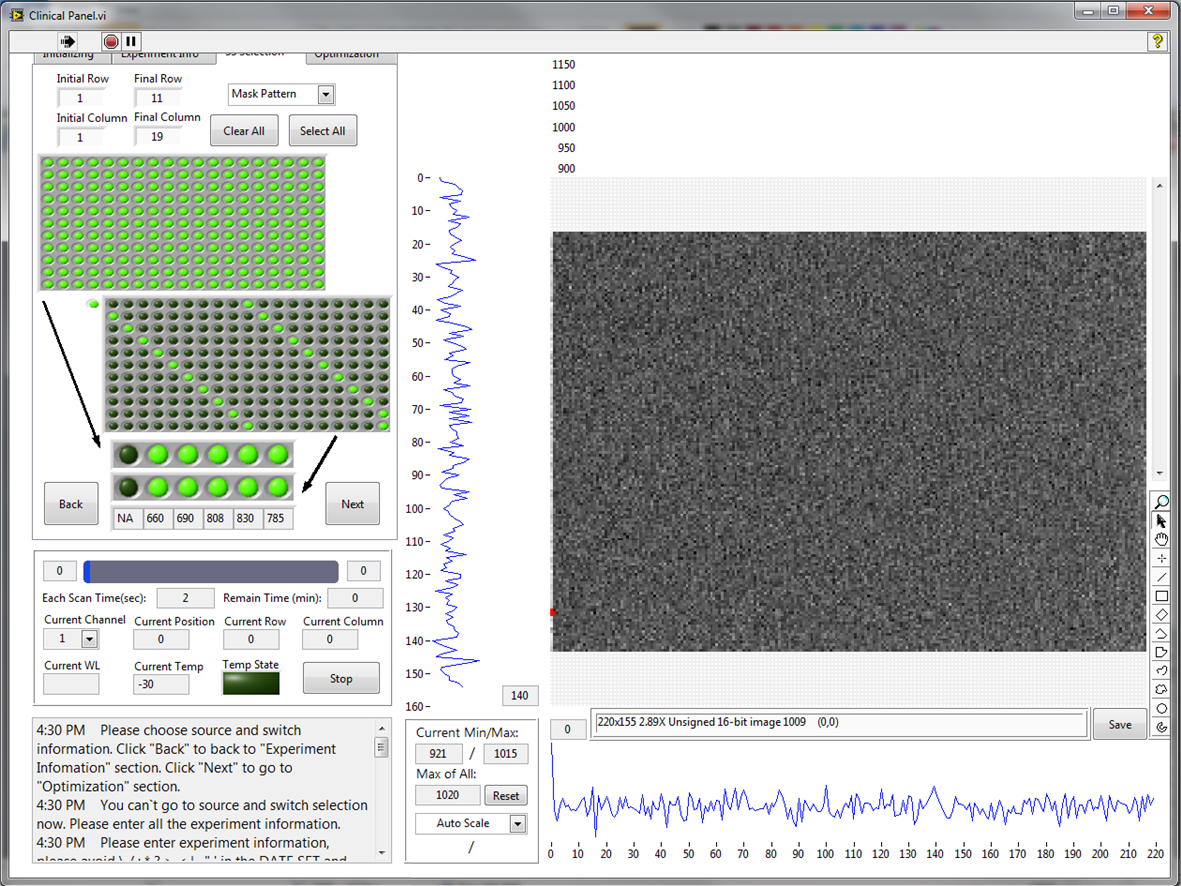
\includegraphics[width=13.5cm]{./figures/A_Gen3Software/Clinical4.png}
\caption[Measurement setup panel in the clinical software]{The third control panel is the source configuration screen. Here the source positions, the calibration measurements, and wavelengths used in the experiment can be chosen.}
\label{fig:Clinical4}
\end{figure}
At this panel, the detection gain and the laser intensities are adjusted so that the CCD not saturated for the particular breast or sourceplate detection window separation distance. The pickoff light level is adjusted at this stage. Note that the pickoff does not go through the imaging tank, so it must be adjusted independently of the laser sources.

The last panel in the clinical software is the measurement panel. At this point, the user can begin the measurements. The steps displayed on this screen is dependent on the entries in the previous panels. The user simply takes the measurement from the top to the bottom. The green light after each measurement description lights up indicating that the measurement is completed.
\vspace{3mm}
\begin{figure}[h]
\centering
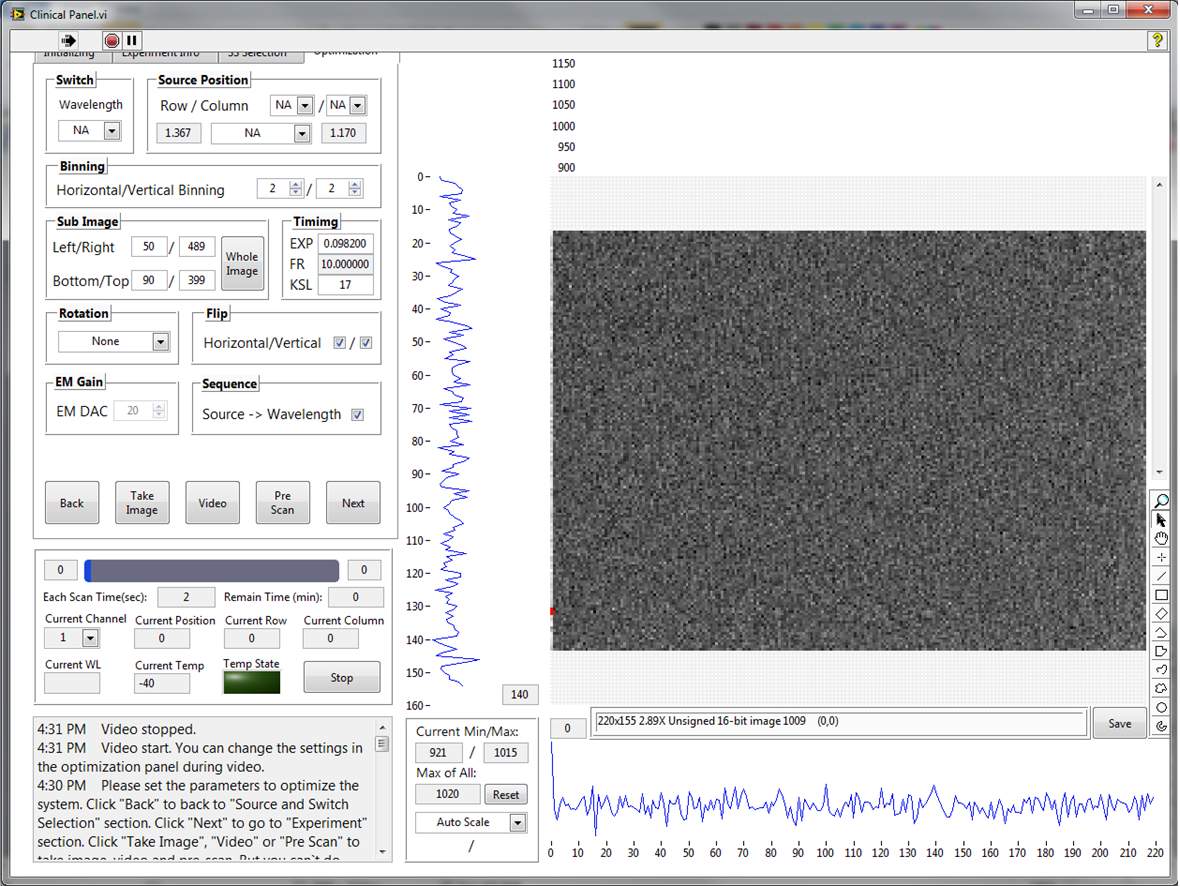
\includegraphics[width=13.5cm]{./figures/A_Gen3Software/Clinical5.png}
\caption[The optimization panel in the clinical software]{The measurement optimization screen. At this stage, the CCD can be run in video mode with the same exposure used in the actual measurements. The laser light level and detection gain is adjusted so that the CCD is not saturated or so that the light level is adequate for the current experiment.}
\label{fig:Clinical5}
\end{figure}
\begin{figure}[t]
\centering
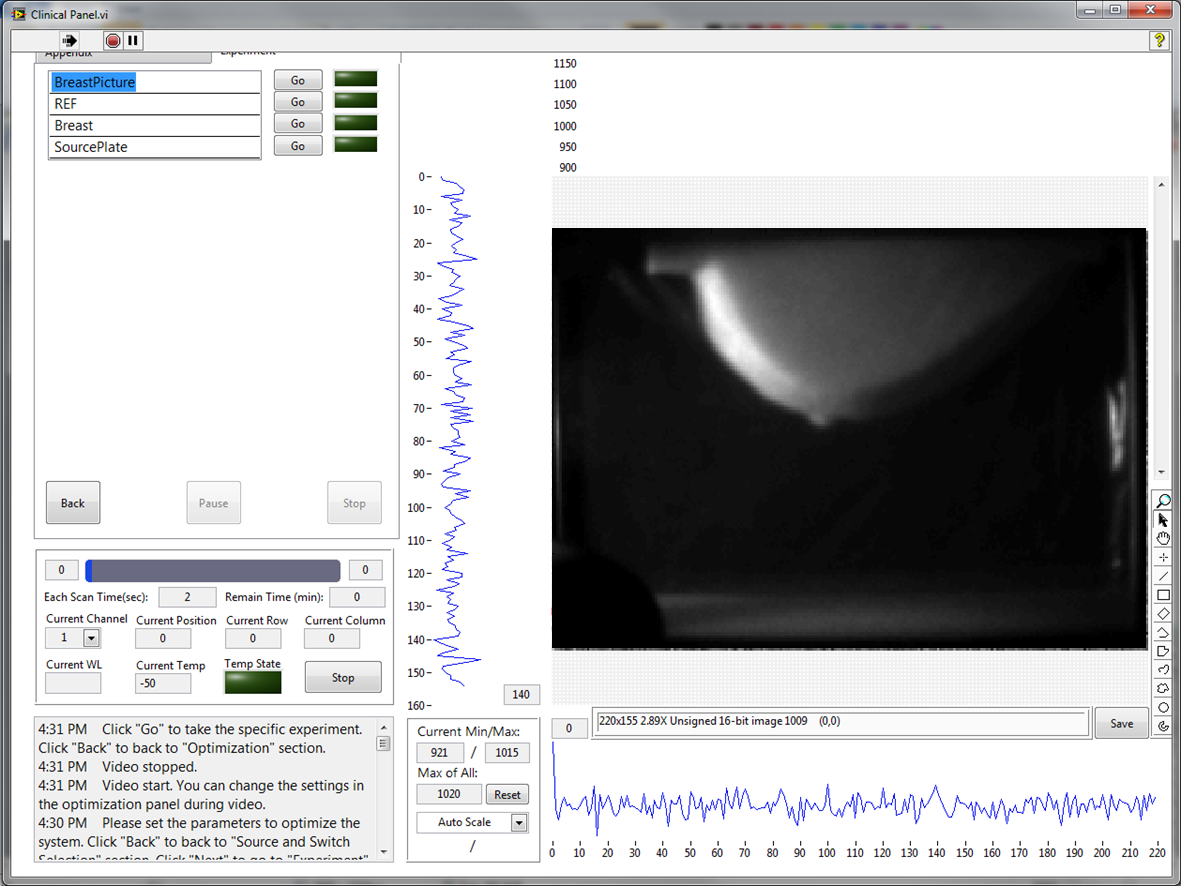
\includegraphics[width=13.5cm]{./figures/A_Gen3Software/Clinical6.png}
\caption[The measurement panel in the clinical software]{The measurement screen of the Gen3 clinical software. After setting up the experiment, the user takes the measurements in series on this screen by pressing the measurement buttons in sequence from top to bottom.}
\label{fig:Clinical6}
\end{figure}